\documentclass[11pt,a4paper]{article}

% ---------- Fonts and page ----------
\usepackage[T1]{fontenc}
\usepackage[utf8]{inputenc}
\usepackage[scaled=0.95]{helvet}
\renewcommand{\familydefault}{\sfdefault}
\usepackage[margin=2.2cm]{geometry}
\usepackage{graphicx}
\usepackage{xcolor}
\usepackage{tikz}
\usetikzlibrary{arrows.meta,positioning,shapes.misc,calc,fit,backgrounds,shadows.blur}
\usepackage[most]{tcolorbox}
\usepackage{enumitem}
\usepackage{booktabs}
\usepackage{caption}
\usepackage{float}
\usepackage{parskip}
\usepackage{hyperref}
\hypersetup{colorlinks=true,linkcolor=navy,urlcolor=navy,pdftitle={Our Family Album: the plan}}

% ---------- Colours ----------
\definecolor{navy}{HTML}{1F3A5F}
\definecolor{sea}{HTML}{2E5A8A}
\definecolor{accent}{HTML}{C8362B}
\definecolor{sand}{HTML}{F5E6B8}
\definecolor{mist}{HTML}{F2F4F7}
\definecolor{ink}{HTML}{1F2937}
\definecolor{muted}{HTML}{6B7280}
\definecolor{line}{HTML}{D9DDE3}
\definecolor{green}{HTML}{2E7D32}
\definecolor{amber}{HTML}{B45309}
\definecolor{ph1}{HTML}{C9773A}
\definecolor{ph2}{HTML}{1F5FA8}
\definecolor{ph3}{HTML}{6C8E4E}
\definecolor{ph4}{HTML}{8B5E83}
\definecolor{ph5}{HTML}{D8B04A}

% ---------- Headings ----------
\usepackage{titlesec}
\titleformat{\section}{\Large\bfseries\color{navy}}{\thesection}{0.8em}{}
\titleformat{\subsection}{\large\bfseries\color{sea}}{\thesubsection}{0.8em}{}
\titlespacing*{\section}{0pt}{14pt}{5pt}
\titlespacing*{\subsection}{0pt}{10pt}{3pt}

% ---------- Boxes ----------
\newtcolorbox{note}[1][Good to know]{enhanced,colback=mist,colframe=sea,boxrule=0.6pt,arc=3pt,
  title=#1,fonttitle=\bfseries,coltitle=white,colbacktitle=sea,left=6pt,right=6pt,top=4pt,bottom=4pt}
\newtcolorbox{privacy}[1][Your privacy]{enhanced,colback=sand!40,colframe=amber,boxrule=0.6pt,arc=3pt,
  title=#1,fonttitle=\bfseries,coltitle=white,colbacktitle=amber,left=6pt,right=6pt,top=4pt,bottom=4pt}

% ---------- Tikz styles ----------
\tikzset{
  box/.style={draw=line,fill=white,rounded corners=3pt,inner sep=6pt,align=center,text=ink,minimum height=1.1cm,blur shadow={shadow blur steps=4,shadow opacity=12}},
  stepbox/.style={box,minimum width=2.6cm,text width=2.6cm,font=\small},
  pill/.style={draw=sea,fill=sea!8,rounded corners=8pt,inner sep=4pt,font=\footnotesize,text=navy},
  arrow/.style={-{Stealth[length=2.5mm]},line width=0.8pt,color=sea},
  thumb/.style={draw=line,fill=#1,rounded corners=2pt,minimum width=9mm,minimum height=9mm,inner sep=0pt},
  phone/.style={draw=ink,line width=1.2pt,rounded corners=14pt,fill=white},
  screen/.style={fill=mist,rounded corners=8pt},
  ui/.style={draw=line,fill=white,rounded corners=3pt,inner sep=3pt,font=\scriptsize,text=ink,align=left},
  btn/.style={fill=navy,text=white,rounded corners=4pt,inner sep=4pt,font=\scriptsize\bfseries},
  btn2/.style={draw=line,fill=white,text=ink,rounded corners=4pt,inner sep=4pt,font=\scriptsize},
  lbl/.style={font=\scriptsize,text=ink,anchor=west,align=left},
  mlbl/.style={font=\scriptsize,text=muted,anchor=west,align=left},
  face/.style={circle,draw=sea,fill=sea!20,minimum size=5mm,inner sep=0pt},
}

% Phone frame macro: \phoneframe{width}{height} draws the frame at the origin; content goes in a scope after it.
\newcommand{\phoneframe}[2]{%
  \draw[phone] (0,0) rectangle (#1,#2);
  \fill[screen] (0.18,0.35) rectangle (#1-0.18,#2-0.35);
  \draw[line,line width=1pt] (#1/2-0.5,#2-0.17) -- (#1/2+0.5,#2-0.17);
  \draw[line,line width=1.2pt,rounded corners=2pt] (#1/2-0.6,0.16) -- (#1/2+0.6,0.16);
}

\captionsetup{font=small,labelfont={bf,color=navy},skip=4pt}
\setlist{nosep,leftmargin=1.4em}

\begin{document}

% ================= Title =================
\begin{center}
  
\begin{tikzpicture}
    \fill[navy,rounded corners=10pt] (0,0) rectangle (16,4.2);
    \fill[sea] (0,0) [rounded corners=10pt] -- (0,1.1) .. controls (4,1.6) and (8,0.6) .. (16,1.3) -- (16,0) -- cycle;
    \fill[sand] (13.6,3.1) circle (0.42);
    \fill[white] (11.9,1.0) -- (12.05,2.6) -- (12.55,2.6) -- (12.7,1.0) -- cycle;
    \fill[accent] (12.0,1.7) rectangle (12.6,1.95);
    \fill[accent] (11.95,1.2) rectangle (12.65,1.45);
    \fill[ink] (12.0,2.6) rectangle (12.6,2.85);
    \fill[sand] (12.1,2.65) rectangle (12.5,2.8);
    \node[anchor=west,text=white,font=\Huge\bfseries] at (0.7,2.75) {Our Family Album};
    \node[anchor=west,text=sand,font=\large] at (0.7,1.85) {What it does today, and where it is going};
    \node[anchor=west,text=white!80,font=\small] at (0.7,1.15) {A plan to share with the family \quad\textbullet\quad September 2026};
  \end{tikzpicture}
\end{center}

\vspace{4pt}
This is a plain-language description of our own photo website, and of the next things we would like to add to it. It is written for everyone in the family, not for programmers. The first part explains what already works. The second part explains the plan: making the album the one place where all our photos and videos live, and making them easy to find again. The last part lists a few questions we should agree on together.

\tableofcontents

% ================= Part 1 =================
\section{What we have today}

\subsection{Your own private website for family trips}

The album is a website that we run ourselves. It is not Facebook, Google Photos or iCloud: the pictures sit on a computer that belongs to the family, and only people we invite can see them. It works in any browser, and on a phone it can be added to the home screen so it opens like an app, with its own icon.

\subsection{Getting in}

There are no passwords to remember. You type your email address, we send you a link, and tapping the link signs you in for about three months on that phone or computer. Only addresses that have been invited can get a link, so a stranger who finds the site gets nothing.

\begin{note}[Installing it on a phone]
\textbf{iPhone:} open the site in Safari, tap Share, then \emph{Add to Home Screen}. \textbf{Android:} open it in Chrome, tap the menu, then \emph{Install app}. It then opens full screen with the lighthouse icon.
\end{note}

\subsection{What you can do}

\begin{itemize}
  \item \textbf{Trips.} Every holiday gets its own page, with its own look: a lighthouse theme for Maine, highlands for Scotland, swamp for the Everglades, and so on.
  \item \textbf{Activities.} Within a trip, hikes, bike rides, boat trips and meals are separate events. A hike recorded on a watch shows its route on a map and the usual numbers: distance, time, climb, heart rate.
  \item \textbf{Timeline.} Every trip can be read day by day, with the photos and activities of each day in order.
  \item \textbf{Map.} Every photo with a location appears on a map, along with the routes we walked, rode or drove.
  \item \textbf{Photos placed automatically.} If a photo has no location but was taken during a recorded hike, the album works out where on the trail you were when you took it.
  \item \textbf{Sharing.} A trip is private unless we decide otherwise. It can be shared with a secret link (for relatives without an account) or made fully public.
\end{itemize}

\begin{figure}[H]
  \centering
  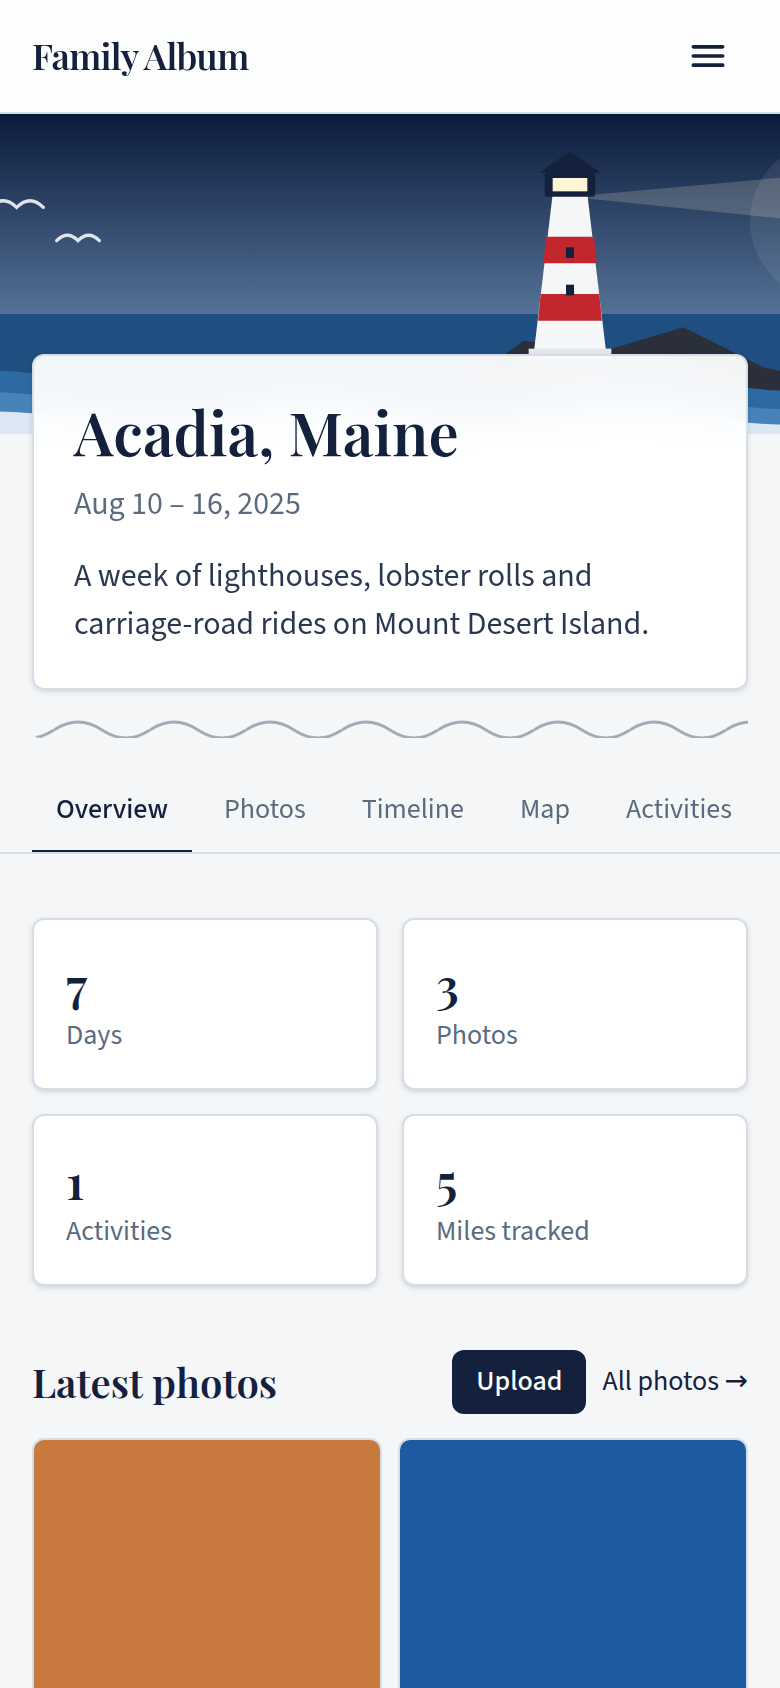
\includegraphics[height=7.2cm]{img/trip.png}\hspace{6pt}
  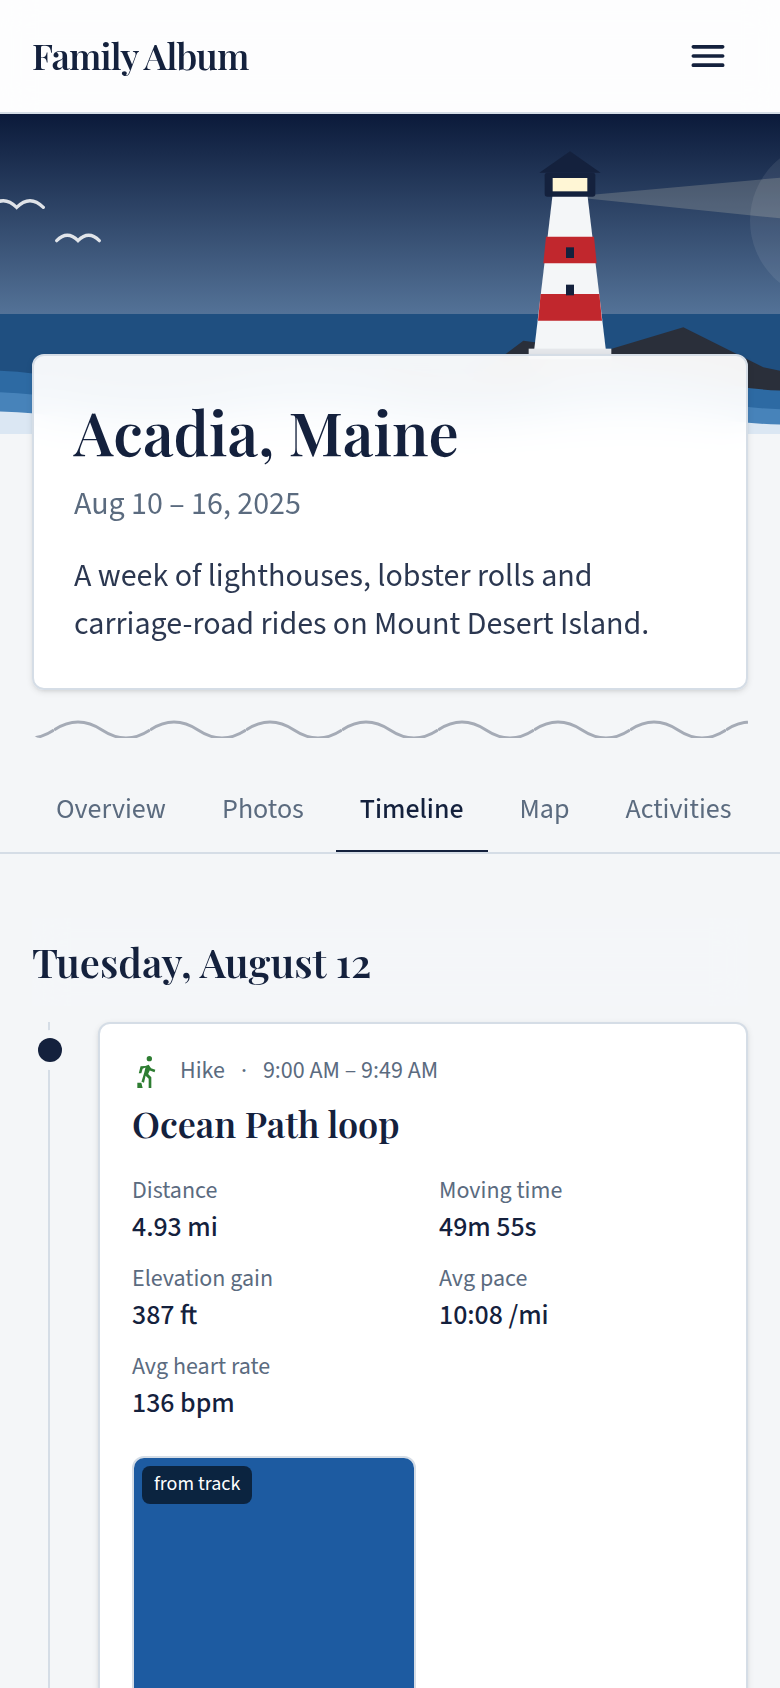
\includegraphics[height=7.2cm]{img/timeline.png}\hspace{6pt}
  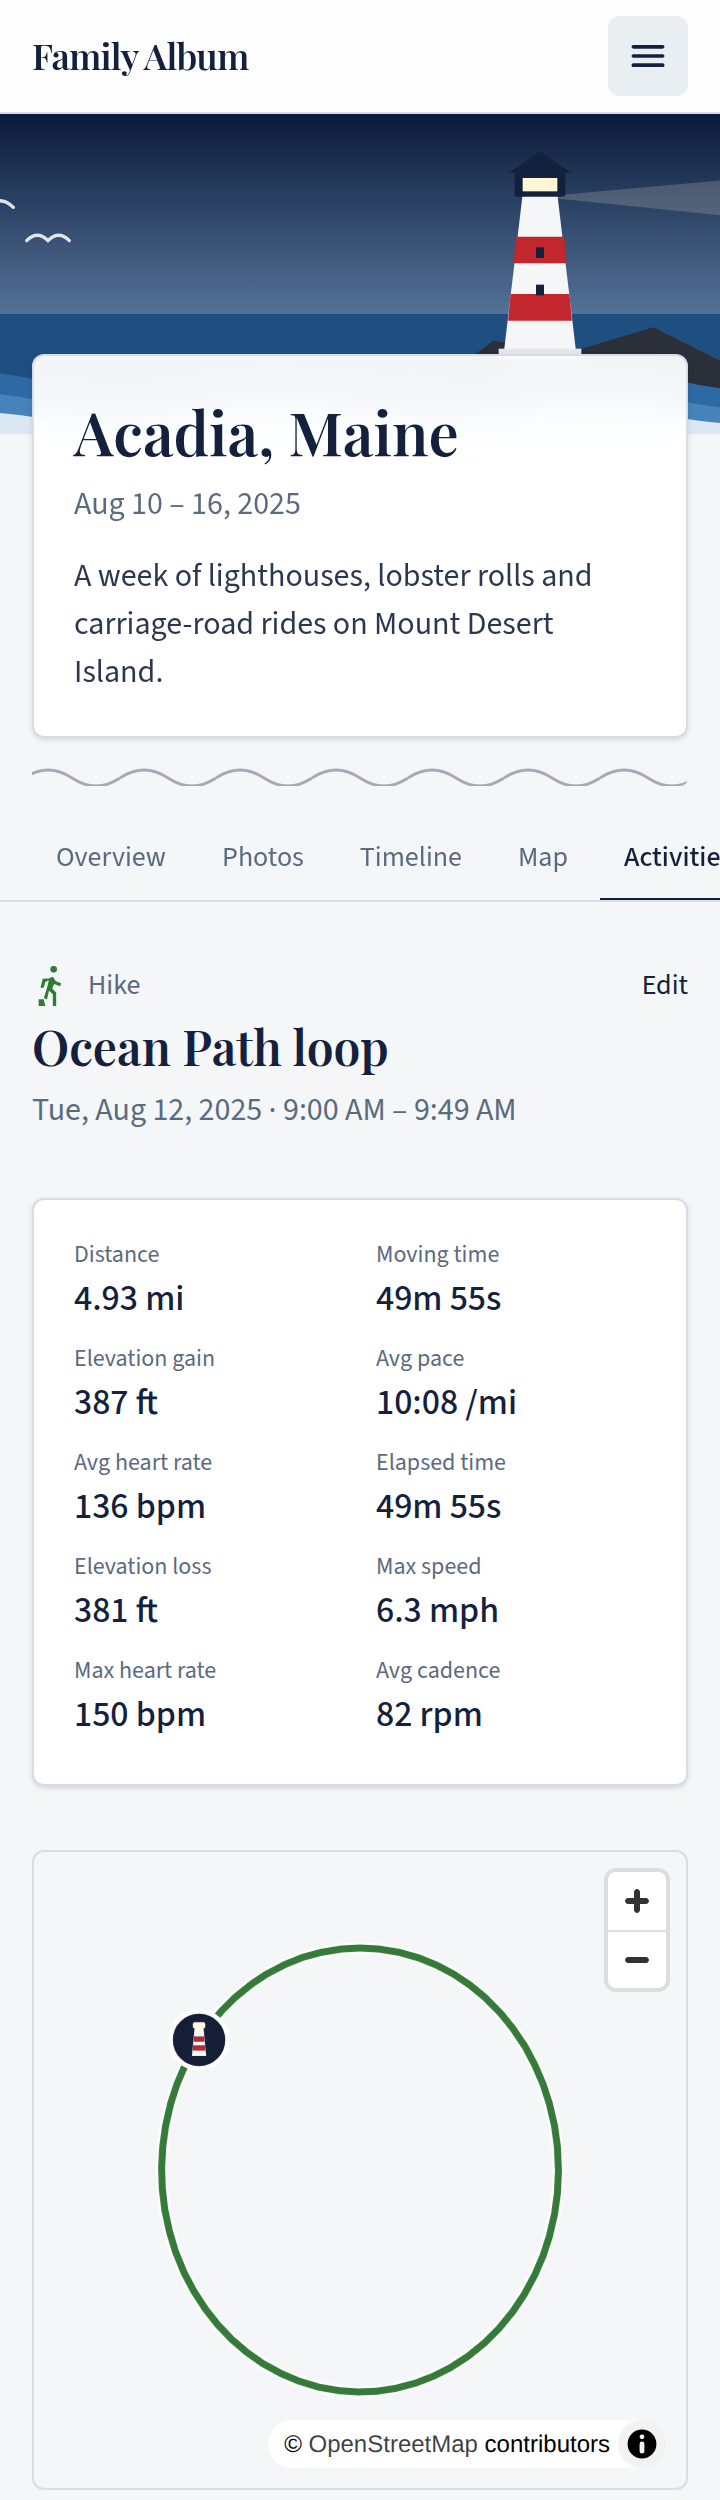
\includegraphics[height=7.2cm]{img/activity.png}
  \caption{The album on a phone today: a trip page with its theme, the day-by-day timeline, and a hike with its route and numbers.}
\end{figure}

% ================= Part 2 =================
\section{The plan: one home for all our photos and videos}

Today the album is organised around trips. The plan is to widen it so that \emph{every} family photo and video can go in, whether or not it belongs to a holiday, and so that anything can be found again years later with a simple search. Here is what changes, from the point of view of someone using it.

\subsection{Trips and collections}

A \textbf{trip} stays what it is: a holiday with dates, places and activities. A \textbf{collection} is new: any set of photos and videos you want to keep together, for any reason. ``Grandma Jo'', ``Every lighthouse we have ever visited'', ``Christmas mornings'', ``Sam growing up''. A photo can belong to one trip, but to as many collections as you like. Collections get their own page, their own theme, and can be shared exactly like a trip.

\begin{figure}[H]
  \centering
  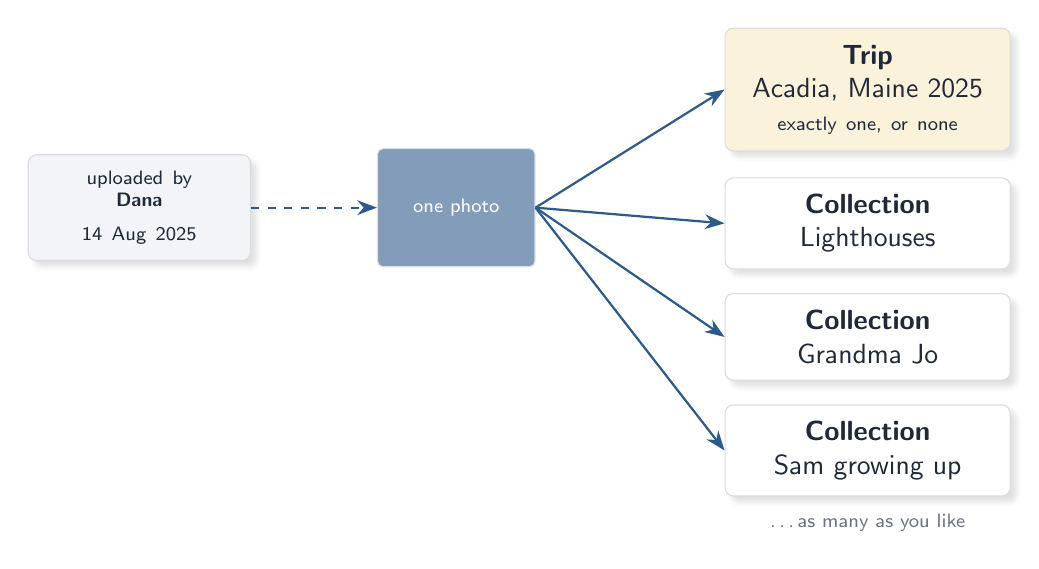
\begin{tikzpicture}[node distance=8mm]
    \node[thumb=sea!60,minimum width=2cm,minimum height=1.5cm] (photo) {\color{white}\scriptsize one photo};
    \node[box,fill=sand!50,right=2.4cm of photo,yshift=1.5cm,text width=3.2cm] (trip) {\textbf{Trip}\\Acadia, Maine 2025\\\scriptsize exactly one, or none};
    \node[box,right=2.4cm of photo,yshift=-0.2cm,text width=3.2cm] (c1) {\textbf{Collection}\\Lighthouses};
    \node[box,below=3mm of c1,text width=3.2cm] (c2) {\textbf{Collection}\\Grandma Jo};
    \node[box,below=3mm of c2,text width=3.2cm] (c3) {\textbf{Collection}\\Sam growing up};
    \node[mlbl,anchor=north] at ($(c3.south)+(0,-1mm)$) {\ldots as many as you like};
    \draw[arrow] (photo.east) -- (trip.west);
    \draw[arrow] (photo.east) -- (c1.west);
    \draw[arrow] (photo.east) -- (c2.west);
    \draw[arrow] (photo.east) -- (c3.west);
    \node[box,left=1.6cm of photo,text width=2.4cm,fill=mist] (who) {\scriptsize uploaded by\\\textbf{Dana}\\\scriptsize 14 Aug 2025};
    \draw[arrow,dashed] (who.east) -- (photo.west);
  \end{tikzpicture}
  \caption{Where a photo can live. It sits on at most one trip, in any number of collections, and always remembers who uploaded it.}
\end{figure}

\begin{figure}[H]
  \centering
  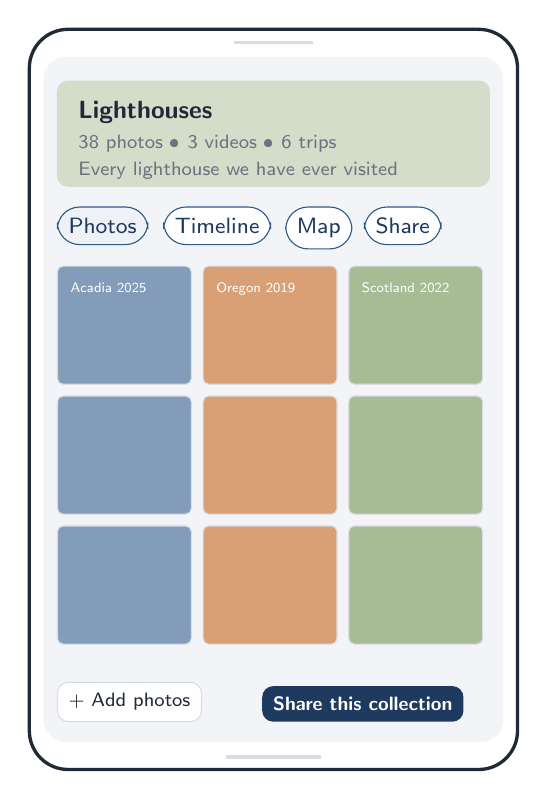
\begin{tikzpicture}[x=1cm,y=1cm]
    \phoneframe{6.2}{9.4}
    \begin{scope}[shift={(0.35,0)}]
      \fill[ph3!30,rounded corners=4pt] (0,7.4) rectangle (5.5,8.75);
      \node[lbl,font=\small\bfseries] at (0.15,8.35) {Lighthouses};
      \node[mlbl] at (0.15,7.95) {38 photos \textbullet\ 3 videos \textbullet\ 6 trips};
      \node[mlbl] at (0.15,7.6) {Every lighthouse we have ever visited};
      \node[pill,anchor=north west] at (0,7.15) {Photos};
      \node[pill,anchor=north west,fill=white] at (1.35,7.15) {Timeline};
      \node[pill,anchor=north west,fill=white] at (2.9,7.15) {Map};
      \node[pill,anchor=north west,fill=white] at (3.9,7.15) {Share};
      \foreach \r in {0,1,2} \foreach \c/\col in {0/sea!60,1/ph1!70,2/ph3!60} {
        \node[thumb=\col,minimum width=1.7cm,minimum height=1.5cm,anchor=north west] at (\c*1.85,6.4-\r*1.65) {};
      }
      \node[mlbl,anchor=north west] at (0.05,6.3) {\tiny\textcolor{white}{Acadia 2025}};
      \node[mlbl,anchor=north west] at (1.9,6.3) {\tiny\textcolor{white}{Oregon 2019}};
      \node[mlbl,anchor=north west] at (3.75,6.3) {\tiny\textcolor{white}{Scotland 2022}};
      \node[btn2,anchor=south west] at (0,0.6) {+ Add photos};
      \node[btn,anchor=south west] at (2.6,0.6) {Share this collection};
    \end{scope}
  \end{tikzpicture}
  \hspace{1cm}
  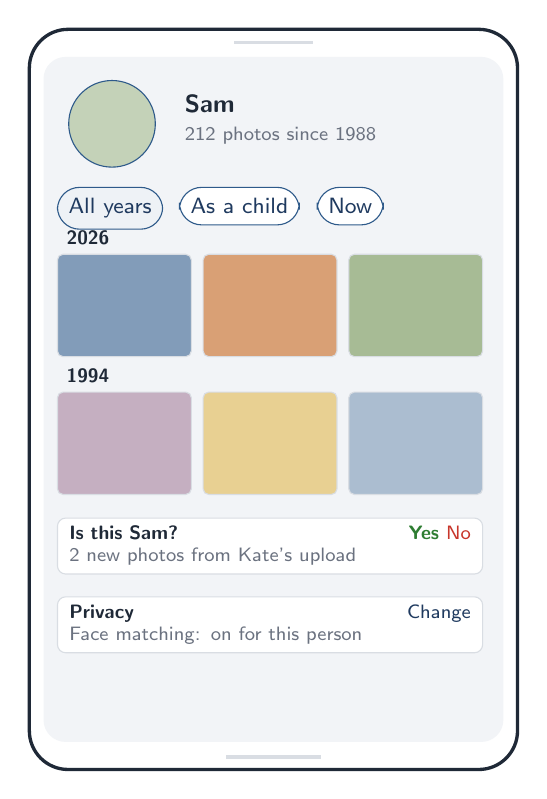
\begin{tikzpicture}[x=1cm,y=1cm]
    \phoneframe{6.2}{9.4}
    \begin{scope}[shift={(0.35,0)}]
      \node[face,minimum size=11mm,fill=ph3!40] at (0.7,8.2) {};
      \node[lbl,font=\small\bfseries] at (1.5,8.45) {Sam};
      \node[mlbl] at (1.5,8.05) {212 photos since 1988};
      \node[pill,anchor=north west] at (0,7.4) {All years};
      \node[pill,anchor=north west,fill=white] at (1.55,7.4) {As a child};
      \node[pill,anchor=north west,fill=white] at (3.3,7.4) {Now};
      \node[lbl,font=\scriptsize\bfseries] at (0,6.75) {2026};
      \foreach \c/\col in {0/sea!60,1/ph1!70,2/ph3!60} {
        \node[thumb=\col,minimum width=1.7cm,minimum height=1.3cm,anchor=north west] at (\c*1.85,6.55) {};
      }
      \node[lbl,font=\scriptsize\bfseries] at (0,5.0) {1994};
      \foreach \c/\col in {0/ph4!50,1/ph5!60,2/sea!40} {
        \node[thumb=\col,minimum width=1.7cm,minimum height=1.3cm,anchor=north west] at (\c*1.85,4.8) {};
      }
      \node[ui,minimum width=5.4cm,anchor=north west,text width=5.1cm] at (0,3.2)
        {\textbf{Is this Sam?} \hfill \textcolor{green}{\textbf{Yes}} \textcolor{accent}{No}\\\textcolor{muted}{2 new photos from Kate's upload}};
      \node[ui,minimum width=5.4cm,anchor=north west,text width=5.1cm] at (0,2.2)
        {\textbf{Privacy} \hfill \textcolor{navy}{Change}\\\textcolor{muted}{Face matching: on for this person}};
    \end{scope}
  \end{tikzpicture}
  \caption{Sketches of a collection page (left) and a person's page (right). A collection can gather photos from many trips; a person's page groups their photos by year and asks about new matches.}
\end{figure}

\subsection{Uploading: from your phone to the album}

Uploading becomes the heart of the site. Everyone can add photos and videos, from a phone or a computer, one at a time or a whole card full. Big videos no longer fail on bad hotel Wi-Fi: an interrupted upload picks up where it stopped.

After the files arrive, you land on a short \textbf{review} screen. This is the one new habit we are asking of everyone: write a sentence or two about what the pictures are. It can be one note for a whole batch (``Nana's 80th at the lake house, everyone came'') rather than one per photo. That sentence is what makes the photos findable later, as the next section explains.

\begin{figure}[H]
  \centering
  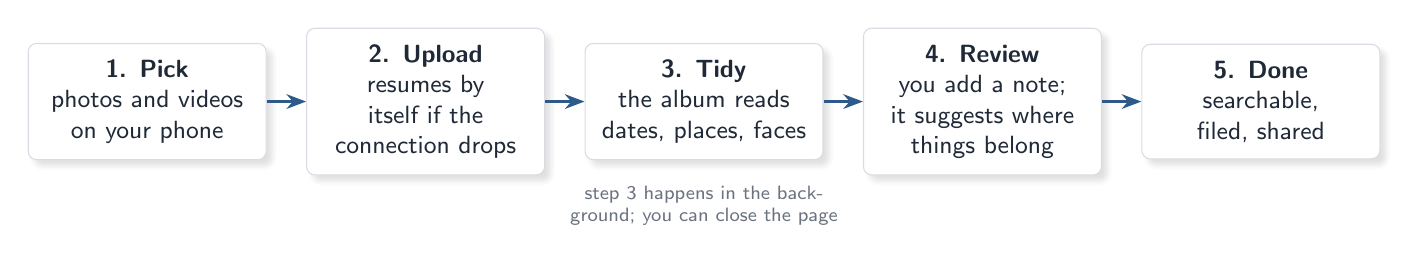
\begin{tikzpicture}[node distance=5mm]
    \node[stepbox] (a) {\textbf{1. Pick}\\photos and videos on your phone};
    \node[stepbox,right=of a] (b) {\textbf{2. Upload}\\resumes by itself if the connection drops};
    \node[stepbox,right=of b] (c) {\textbf{3. Tidy}\\the album reads dates, places, faces};
    \node[stepbox,right=of c] (d) {\textbf{4. Review}\\you add a note; it suggests where things belong};
    \node[stepbox,right=of d] (e) {\textbf{5. Done}\\searchable, filed, shared};
    \foreach \x/\y in {a/b,b/c,c/d,d/e} \draw[arrow] (\x) -- (\y);
    \node[mlbl,anchor=north,text width=6cm,align=center] at ($(c.south)+(0,-2mm)$) {step 3 happens in the background; you can close the page};
  \end{tikzpicture}
  \caption{The five steps of adding something to the album. Only steps 1 and 4 need you.}
\end{figure}

\begin{figure}[H]
  \centering
  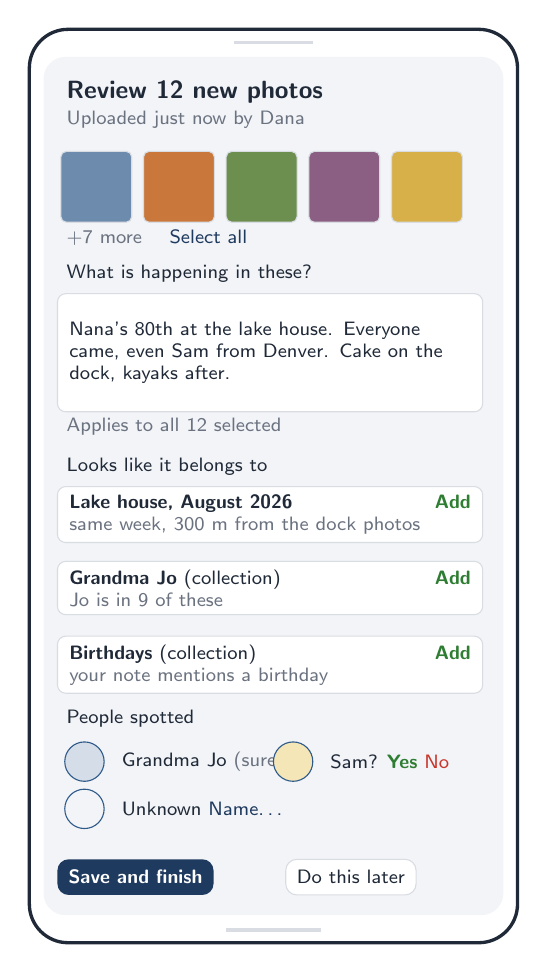
\begin{tikzpicture}[x=1cm,y=1cm]
    \phoneframe{6.2}{11.6}
    \begin{scope}[shift={(0.35,0)}]
      \node[lbl,font=\small\bfseries] at (0,10.8) {Review 12 new photos};
      \node[mlbl] at (0,10.45) {Uploaded just now by Dana};
      % thumbnails row
      \foreach \i/\c in {0/sea!70,1/ph1,2/ph3,3/ph4,4/ph5} {
        \node[thumb=\c] at (0.5+\i*1.05,9.6) {};
      }
      \node[mlbl] at (0,8.95) {+7 more \quad \textcolor{navy}{Select all}};
      % context box
      \node[lbl] at (0,8.5) {What is happening in these?};
      \node[ui,minimum width=5.4cm,minimum height=1.5cm,anchor=north west,text width=5.1cm] at (0,8.25)
        {Nana's 80th at the lake house. Everyone came, even Sam from Denver. Cake on the dock, kayaks after.};
      \node[mlbl] at (0,6.55) {Applies to all 12 selected};
      % suggestions
      \node[lbl] at (0,6.05) {Looks like it belongs to};
      \node[ui,minimum width=5.4cm,anchor=north west,text width=5.1cm] at (0,5.8)
        {\textbf{Lake house, August 2026} \hfill \textcolor{green}{\textbf{Add}}\\\textcolor{muted}{same week, 300 m from the dock photos}};
      \node[ui,minimum width=5.4cm,anchor=north west,text width=5.1cm] at (0,4.85)
        {\textbf{Grandma Jo} (collection) \hfill \textcolor{green}{\textbf{Add}}\\\textcolor{muted}{Jo is in 9 of these}};
      \node[ui,minimum width=5.4cm,anchor=north west,text width=5.1cm] at (0,3.9)
        {\textbf{Birthdays} (collection) \hfill \textcolor{green}{\textbf{Add}}\\\textcolor{muted}{your note mentions a birthday}};
      % people
      \node[lbl] at (0,2.85) {People spotted};
      \node[face] at (0.35,2.3) {};
      \node[lbl] at (0.7,2.3) {Grandma Jo \textcolor{muted}{(sure)}};
      \node[face,fill=sand] at (3.0,2.3) {};
      \node[lbl] at (3.35,2.3) {Sam? \textcolor{green}{\textbf{Yes}} \textcolor{accent}{No}};
      \node[face,fill=mist] at (0.35,1.7) {};
      \node[lbl] at (0.7,1.7) {Unknown \textcolor{navy}{Name\ldots}};
      \node[btn,anchor=south west] at (0,0.6) {Save and finish};
      \node[btn2,anchor=south west] at (2.9,0.6) {Do this later};
    \end{scope}
  \end{tikzpicture}
  \caption{The review screen after an upload (a sketch, not the final design). One note covers the whole batch; suggested trips and collections come with a reason; faces the album recognises are offered for a yes or no.}
\end{figure}

\subsection{Videos too}

Videos come in two kinds, and they take two different routes.

\textbf{Short clips} (up to about a minute) are uploaded straight into the album like photos. They play silently in the photo grid when you tap or hover, the way stories do on social apps, and with sound and controls when opened. They are converted so they play on any phone or computer, and the original file is kept.

\textbf{Longer videos} (the school play, the whole wedding speech) are not uploaded to the album. Instead, whoever has the video puts it on YouTube as an \emph{unlisted} video, then pastes the YouTube link into the album. The album fetches the title and a still frame, and the video appears in the trip or collection like any other item: it shows up on the timeline, can be given a note, can be searched, and can be added to collections. Pressing play on it plays the video right there on the page. Unlisted means the video does not appear in YouTube searches or on anyone's channel; only people with the link can watch it. YouTube does the heavy lifting of storing and streaming, which keeps our own computer small.

\begin{figure}[H]
  \centering
  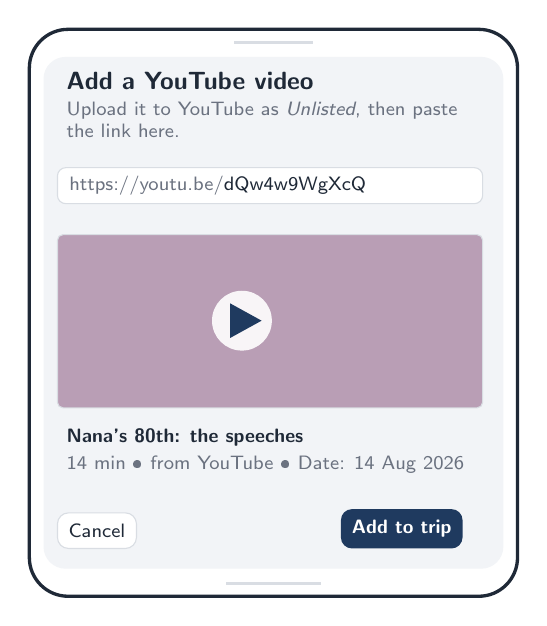
\begin{tikzpicture}[x=1cm,y=1cm]
    \phoneframe{6.2}{7.2}
    \begin{scope}[shift={(0.35,0)}]
      \node[lbl,font=\small\bfseries] at (0,6.55) {Add a YouTube video};
      \node[mlbl,text width=5.2cm] at (0,6.05) {Upload it to YouTube as \emph{Unlisted}, then paste the link here.};
      \node[ui,minimum width=5.4cm,anchor=north west,text width=5.1cm] at (0,5.45) {\textcolor{muted}{https://youtu.be/}dQw4w9WgXcQ};
      \node[thumb=ph4!60,minimum width=5.4cm,minimum height=2.2cm,anchor=north west] at (0,4.6) {};
      \fill[white,opacity=0.9] (2.35,3.5) circle (0.38);
      \fill[navy] (2.2,3.28) -- (2.2,3.72) -- (2.6,3.5) -- cycle;
      \node[lbl,anchor=north west] at (0,2.25) {\textbf{Nana's 80th: the speeches}};
      \node[mlbl,anchor=north west] at (0,1.9) {14 min \textbullet\ from YouTube \textbullet\ Date: 14 Aug 2026};
      \node[btn2,anchor=south west] at (0,0.6) {Cancel};
      \node[btn,anchor=south west] at (3.6,0.6) {Add to trip};
    \end{scope}
  \end{tikzpicture}
  \hspace{0.8cm}
  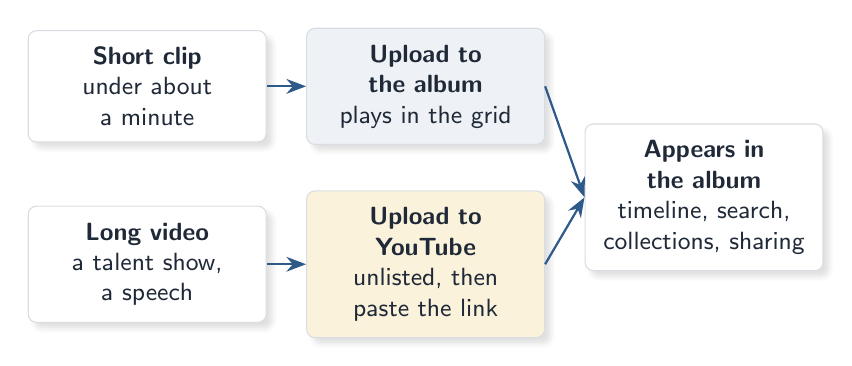
\begin{tikzpicture}[node distance=5mm]
    \node[stepbox,text width=2.6cm] (a) {\textbf{Short clip}\\under about a minute};
    \node[stepbox,text width=2.6cm,below=8mm of a] (b) {\textbf{Long video}\\a talent show, a speech};
    \node[stepbox,text width=2.6cm,right=of a,fill=sea!8] (a2) {\textbf{Upload to the album}\\plays in the grid};
    \node[stepbox,text width=2.6cm,right=of b,fill=sand!50] (b2) {\textbf{Upload to YouTube}\\unlisted, then paste the link};
    \node[stepbox,text width=2.6cm,right=of b2,yshift=8.5mm] (c) {\textbf{Appears in the album}\\timeline, search, collections, sharing};
    \draw[arrow] (a) -- (a2); \draw[arrow] (b) -- (b2);
    \draw[arrow] (a2.east) -- (c.west); \draw[arrow] (b2.east) -- (c.west);
  \end{tikzpicture}
  \caption{Left: a sketch of adding a YouTube video by pasting its link. Right: short clips are uploaded; long videos go through YouTube; both end up in the album the same way.}
\end{figure}

\begin{note}[About unlisted YouTube videos]
An unlisted video is hidden from searches and from your channel, but anyone who has its link can watch it, and YouTube keeps a copy on its servers. If a video should stay strictly within the family, keep it as a short clip in the album, or split it into a few clips. The album shows a small reminder about this whenever a YouTube video is added.
\end{note}

\subsection{Bringing photos over from Google Photos}

Many of us already keep photos in Google Photos, and there are two ways to get them into the album. Google no longer lets outside apps read a whole library or copy new photos automatically in the background, so neither route is a permanent link; both are things you do when you want to.

\begin{itemize}
  \item \textbf{A handful at a time.} An \emph{Import from Google Photos} button opens Google's own picking screen. You tick the photos you want, and they arrive in the album as if you had uploaded them, complete with the review screen, notes and suggestions. Each person connects their own Google account once. One catch: Google removes the location from photos it hands over this way, so those photos only land on the map if a recorded hike or drive covers them, or if someone sets the place by hand.
  \item \textbf{Everything at once.} For the big transfer, Google's \emph{Takeout} service packages up an entire library. Those files keep everything, including locations, the captions you typed in Google Photos, and which Google album each photo was in. The album reads them, skips photos we already have, and turns each Google album into a collection. The files are large, so they go straight onto the family computer rather than through a phone.
\end{itemize}

\begin{figure}[H]
  \centering
  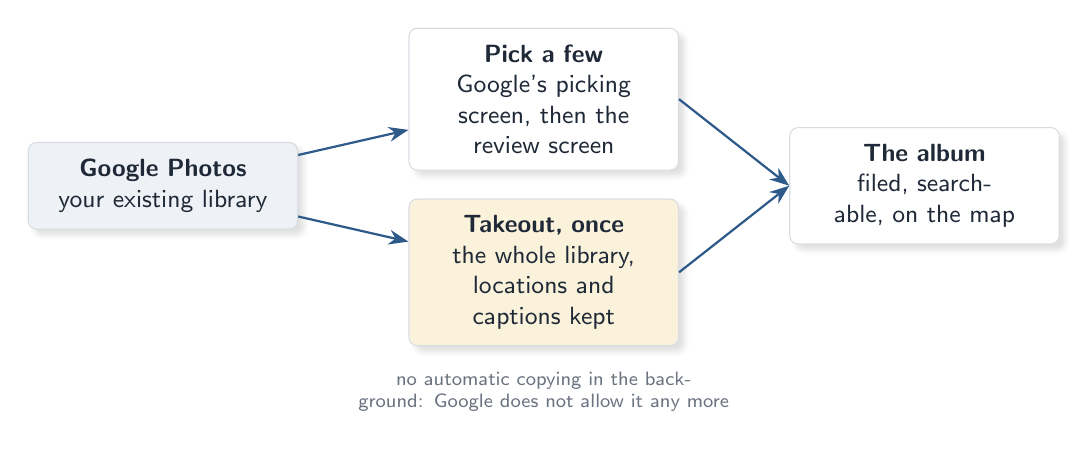
\begin{tikzpicture}[node distance=6mm]
    \node[stepbox,text width=3cm,fill=sea!8] (g) {\textbf{Google Photos}\\your existing library};
    \node[stepbox,text width=3cm,right=1.4cm of g,yshift=1.1cm] (pick) {\textbf{Pick a few}\\Google's picking screen, then the review screen};
    \node[stepbox,text width=3cm,right=1.4cm of g,yshift=-1.1cm,fill=sand!50] (take) {\textbf{Takeout, once}\\the whole library, locations and captions kept};
    \node[stepbox,text width=3cm,right=1.4cm of pick,yshift=-1.1cm] (album) {\textbf{The album}\\filed, searchable, on the map};
    \draw[arrow] (g) -- (pick); \draw[arrow] (g) -- (take);
    \draw[arrow] (pick.east) -- (album.west); \draw[arrow] (take.east) -- (album.west);
    \node[mlbl,anchor=north,text width=8cm,align=center] at ($(take.south)+(0,-2mm)$) {no automatic copying in the background: Google does not allow it any more};
  \end{tikzpicture}
  \caption{Two ways in from Google Photos: pick a few when you need them, or bring the whole library over once with Takeout.}
\end{figure}

\subsection{Finding anything again}

Today you find a photo by remembering which trip it was on. The plan adds a proper search box. You will be able to type things like \emph{``lobster rolls on the boat''}, \emph{``Sam and Kate at Christmas''} or \emph{``the red barn''} and get the right photos, even ones nobody captioned by hand.

This works because of a helper: an AI service that looks at each new photo together with the note you wrote, and writes a short description, a list of what is in the picture, the place, the season and the mood. That description is what search reads. Your note matters a great deal: the helper is good at seeing ``a woman on a dock with a cake'' but cannot know it was Nana's 80th unless someone says so.

\begin{figure}[H]
  \centering
  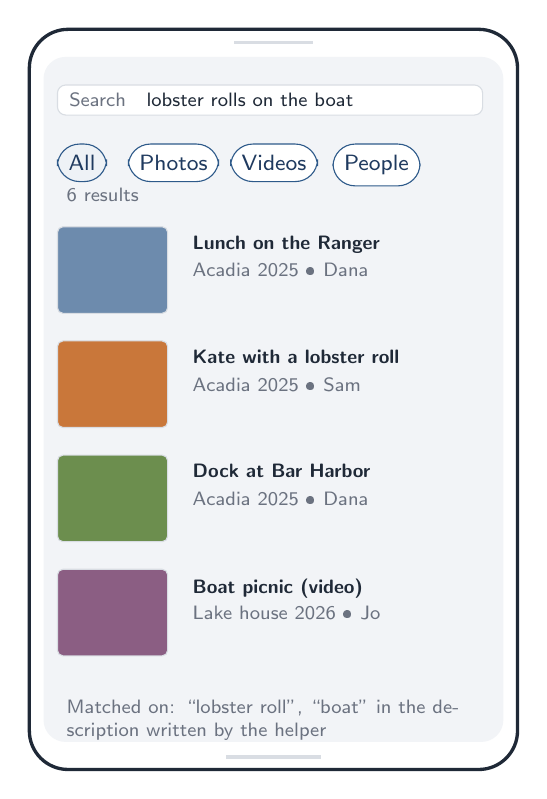
\begin{tikzpicture}[x=1cm,y=1cm]
    \phoneframe{6.2}{9.4}
    \begin{scope}[shift={(0.35,0)}]
      \node[ui,minimum width=5.4cm,anchor=north west,text width=5.1cm] at (0,8.7) {\textcolor{muted}{Search}\quad lobster rolls on the boat};
      \node[pill,anchor=north west] at (0,7.95) {All};
      \node[pill,anchor=north west,fill=white] at (0.9,7.95) {Photos};
      \node[pill,anchor=north west,fill=white] at (2.2,7.95) {Videos};
      \node[pill,anchor=north west,fill=white] at (3.5,7.95) {People};
      \node[mlbl] at (0,7.3) {6 results};
      \foreach \i/\c/\t/\d in {0/sea!70/Lunch on the Ranger/{Acadia 2025 \textbullet\ Dana}, 1/ph1/Kate with a lobster roll/{Acadia 2025 \textbullet\ Sam}, 2/ph3/Dock at Bar Harbor/{Acadia 2025 \textbullet\ Dana}, 3/ph4/Boat picnic (video)/{Lake house 2026 \textbullet\ Jo}} {
        \node[thumb=\c,minimum width=1.4cm,minimum height=1.1cm,anchor=north west] (r\i) at (0,6.9-\i*1.45) {};
        \node[lbl,anchor=north west] at (1.6,6.9-\i*1.45) {\textbf{\t}};
        \node[mlbl,anchor=north west] at (1.6,6.55-\i*1.45) {\d};
      }
      \node[mlbl,anchor=north west,text width=5.1cm] at (0,1.0) {Matched on: ``lobster roll'', ``boat'' in the description written by the helper};
    \end{scope}
  \end{tikzpicture}
  \hspace{1cm}
  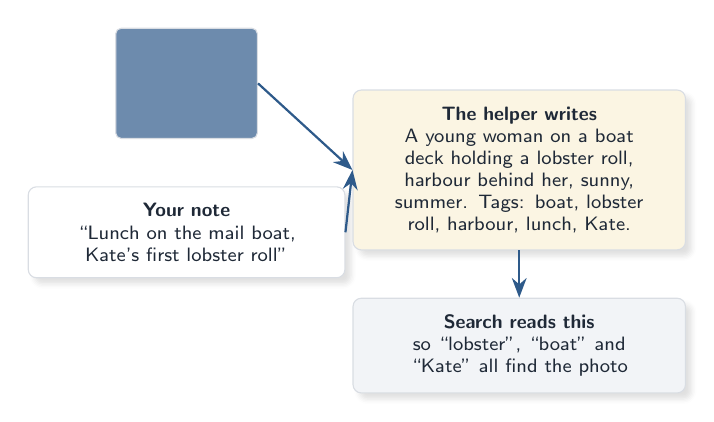
\begin{tikzpicture}[node distance=6mm]
    \node[thumb=sea!70,minimum width=1.8cm,minimum height=1.4cm] (p) {};
    \node[box,below=of p,text width=3.6cm,font=\scriptsize] (n) {\textbf{Your note}\\``Lunch on the mail boat, Kate's first lobster roll''};
    \node[box,right=1.2cm of p,yshift=-1.1cm,text width=3.8cm,font=\scriptsize,fill=sand!40] (ai) {\textbf{The helper writes}\\A young woman on a boat deck holding a lobster roll, harbour behind her, sunny, summer. Tags: boat, lobster roll, harbour, lunch, Kate.};
    \node[box,below=of ai,text width=3.8cm,font=\scriptsize,fill=mist] (s) {\textbf{Search reads this}\\so ``lobster'', ``boat'' and ``Kate'' all find the photo};
    \draw[arrow] (p.east) -- (ai.west);
    \draw[arrow] (n.east) -- (ai.west);
    \draw[arrow] (ai) -- (s);
  \end{tikzpicture}
  \caption{Left: what search will look like. Right: how a photo becomes findable. The photo and your note go in; a description comes out; search reads the description.}
\end{figure}

\subsection{Who is in the picture}

The album will learn to recognise the family. The first time, it groups the faces it finds and asks you to put a name to each group once. After that, when a new photo comes in, it says ``Probably Sam?'' and you confirm with a tap. Every person gets their own page with their photos over the years, and search understands names.

\begin{figure}[H]
  \centering
  
\begin{tikzpicture}[node distance=5mm]
    \node[stepbox,text width=2.5cm] (a) {\textbf{Faces found}\\in new photos};
    \node[stepbox,text width=2.5cm,right=of a] (b) {\textbf{Grouped}\\``the same person appears 40 times''};
    \node[stepbox,text width=2.5cm,right=of b] (c) {\textbf{You name it}\\once: ``Sam''};
    \node[stepbox,text width=2.5cm,right=of c] (d) {\textbf{Next upload}\\``Probably Sam?'' Yes / No};
    \node[stepbox,text width=2.5cm,right=of d] (e) {\textbf{Sam's page}\\and search by name};
    \foreach \x/\y in {a/b,b/c,c/d,d/e} \draw[arrow] (\x) -- (\y);
    \node[mlbl,anchor=north,text width=7cm,align=center] at ($(c.south)+(0,-2mm)$) {a ``No'' is remembered, so the same mistake is not made twice};
  \end{tikzpicture}
  \caption{How naming people works. You name each person once; after that it is a yes or no.}
\end{figure}

\textbf{Old photos of people who are grown up now.} A lot of what we will scan in is the adults of today as children. Faces change so much between five and thirty-five that the album treats each stretch of someone's life as its own group: ``Sam as a small child'', ``Sam as a teenager'', ``Sam now''. Naming a group of childhood faces ``Sam'' simply files it under the Sam that already exists. For old prints with no date, the note you write (``Nana's house, summers around 1990'') tells the album roughly when it was taken, and the album shows its guess for you to confirm. Children who look alike, as siblings often do, always get a ``are you sure?'' before a name sticks.

\begin{figure}[H]
  \centering
  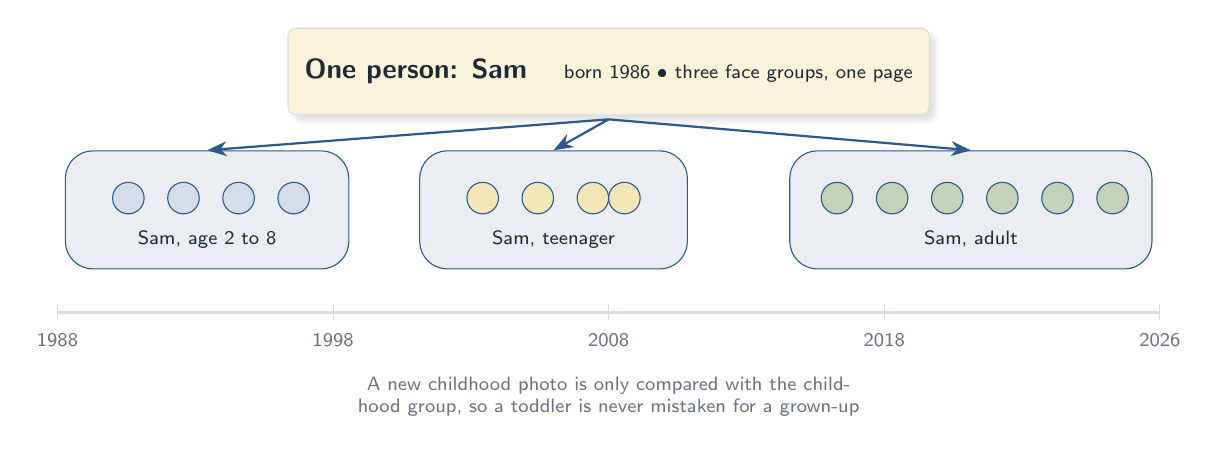
\begin{tikzpicture}
    \draw[line width=1pt,color=line] (0,0) -- (14,0);
    \foreach \x/\y in {0/1988,3.5/1998,7/2008,10.5/2018,14/2026} {
      \draw[line] (\x,-0.1) -- (\x,0.1);
      \node[mlbl,anchor=north,align=center] at (\x,-0.15) {\y};
    }
    \node[draw=sea,fill=sea!10,rounded corners=10pt,minimum width=3.6cm,minimum height=1.5cm] (e1) at (1.9,1.3) {};
    \node[draw=sea,fill=sea!10,rounded corners=10pt,minimum width=3.4cm,minimum height=1.5cm] (e2) at (6.3,1.3) {};
    \node[draw=sea,fill=sea!10,rounded corners=10pt,minimum width=4.6cm,minimum height=1.5cm] (e3) at (11.6,1.3) {};
    \foreach \x in {0.9,1.6,2.3,3.0} \node[face,minimum size=4mm] at (\x,1.45) {};
    \foreach \x in {5.4,6.1,6.8,7.2} \node[face,minimum size=4mm,fill=sand] at (\x,1.45) {};
    \foreach \x in {9.9,10.6,11.3,12.0,12.7,13.4} \node[face,minimum size=4mm,fill=ph3!40] at (\x,1.45) {};
    \node[lbl,anchor=north,align=center] at (1.9,1.15) {\scriptsize Sam, age 2 to 8};
    \node[lbl,anchor=north,align=center] at (6.3,1.15) {\scriptsize Sam, teenager};
    \node[lbl,anchor=north,align=center] at (11.6,1.15) {\scriptsize Sam, adult};
    \node[box,fill=sand!50,anchor=south] at (7,2.5) {\textbf{One person: Sam} \quad\scriptsize born 1986 \textbullet\ three face groups, one page};
    \draw[arrow] (7,2.45) -- (e1.north);
    \draw[arrow] (7,2.45) -- (e2.north);
    \draw[arrow] (7,2.45) -- (e3.north);
    \node[mlbl,anchor=north,text width=8cm,align=center] at (7,-0.7) {A new childhood photo is only compared with the childhood group, so a toddler is never mistaken for a grown-up};
  \end{tikzpicture}
  \caption{One person, several eras. The album keeps a face group per stretch of life and uses the photo's date to pick the right one.}
\end{figure}

\textbf{Pets.} The face matching only knows human faces, so the dog and the cats get their own arrangement. Each pet gets a page like a person, with the years they were with us. The album spots animals in photos and compares the whole animal, not a face, with the photos you have already confirmed, so a distinctive dog or cat is offered as ``Probably Biscuit?'' just like a person. Two black cats will still get mixed up now and then, and the chickens are treated as a flock rather than as individuals, unless one hen is recognisable enough to be named by hand.

\subsection{Who uploaded what}

Every photo already remembers who added it. The plan shows that on each photo, lets you filter a trip or a search by person (``show me what Kate uploaded''), and gives a little count on the admin page so we can see who has been busy scanning the shoeboxes.

\subsection{The photo web}

A more playful addition: a page where photos are laid out as a web, with lines between pictures that look alike. Sunsets drift together, the dog appears as his own cluster, every Christmas tree finds the others. You can look at the web for one trip, one collection or one person, drag it around, and tap any picture to open it. It is a good way to stumble on photos you had forgotten.

\begin{figure}[H]
  \centering
  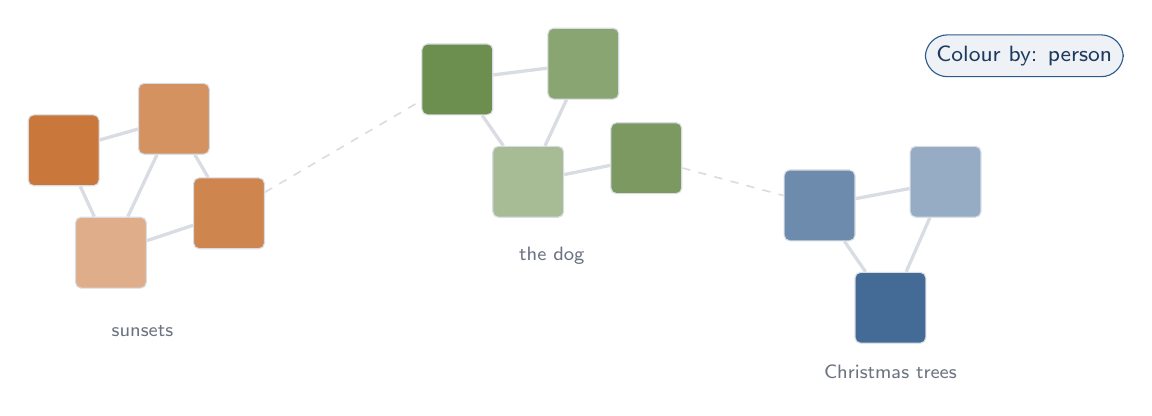
\begin{tikzpicture}
    \coordinate (c1) at (2,2.2); \coordinate (c2) at (7,3.2); \coordinate (c3) at (11.5,1.6);
    % edges first
    \foreach \a/\b in {a1/a2,a1/a3,a2/a3,a3/a4,a2/a4,b1/b2,b2/b3,b1/b3,b3/b4,c1n/c2n,c2n/c3n,c1n/c3n,a4/b1,b4/c1n} {}
    \node[thumb=ph1] (a1) at (1.0,3.0) {};
    \node[thumb=ph1!80] (a2) at (2.4,3.4) {};
    \node[thumb=ph1!60] (a3) at (1.6,1.7) {};
    \node[thumb=ph1!90] (a4) at (3.1,2.2) {};
    \node[thumb=ph3] (b1) at (6.0,3.9) {};
    \node[thumb=ph3!80] (b2) at (7.6,4.1) {};
    \node[thumb=ph3!60] (b3) at (6.9,2.6) {};
    \node[thumb=ph3!90] (b4) at (8.4,2.9) {};
    \node[thumb=sea!70] (c1n) at (10.6,2.3) {};
    \node[thumb=sea!50] (c2n) at (12.2,2.6) {};
    \node[thumb=sea!90] (c3n) at (11.5,1.0) {};
    \begin{scope}[on background layer]
      \foreach \a/\b in {a1/a2,a1/a3,a2/a3,a3/a4,a2/a4,b1/b2,b2/b3,b1/b3,b3/b4,c1n/c2n,c2n/c3n,c1n/c3n} \draw[line width=1.2pt,color=line] (\a) -- (\b);
      \draw[line width=0.6pt,color=line,dashed] (a4) -- (b1);
      \draw[line width=0.6pt,color=line,dashed] (b4) -- (c1n);
    \end{scope}
    \node[mlbl,anchor=north,align=center] at (2,0.9) {sunsets};
    \node[mlbl,anchor=north,align=center] at (7.2,1.9) {the dog};
    \node[mlbl,anchor=north,align=center] at (11.5,0.4) {Christmas trees};
    \node[pill] at (13.2,4.2) {Colour by: person};
  \end{tikzpicture}
  \caption{The photo web. Thick lines join pictures that look alike; clusters form on their own.}
\end{figure}

\subsection{Sharing}

Nothing changes in how sharing works; collections simply get the same three settings as trips.

\begin{figure}[H]
  \centering
  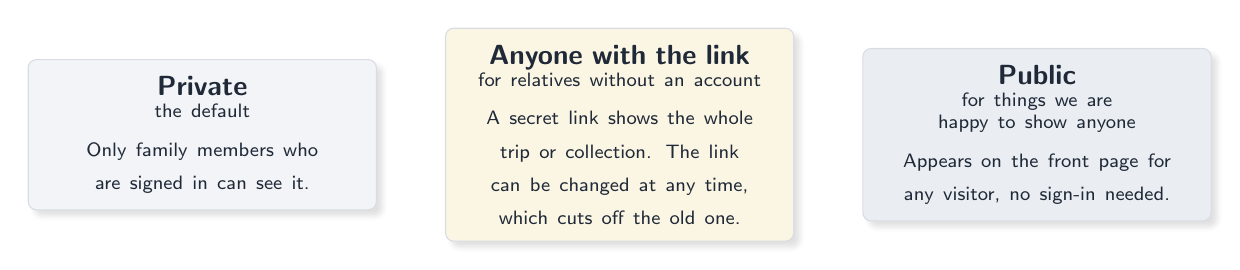
\begin{tikzpicture}
    \node[box,text width=4cm,fill=mist] (p) at (0,0) {\textbf{Private}\\\scriptsize the default\\[2pt]\scriptsize Only family members who are signed in can see it.};
    \node[box,text width=4cm,fill=sand!40] (l) at (5.3,0) {\textbf{Anyone with the link}\\\scriptsize for relatives without an account\\[2pt]\scriptsize A secret link shows the whole trip or collection. The link can be changed at any time, which cuts off the old one.};
    \node[box,text width=4cm,fill=sea!10] (u) at (10.6,0) {\textbf{Public}\\\scriptsize for things we are happy to show anyone\\[2pt]\scriptsize Appears on the front page for any visitor, no sign-in needed.};
  \end{tikzpicture}
  \caption{The three sharing settings. A trip or collection is private unless someone changes it.}
\end{figure}

% ================= Privacy =================
\section{Privacy: what stays home and what does not}

Two parts of the plan use software that looks at the pictures. Here is where the pictures go.

\begin{figure}[H]
  \centering
  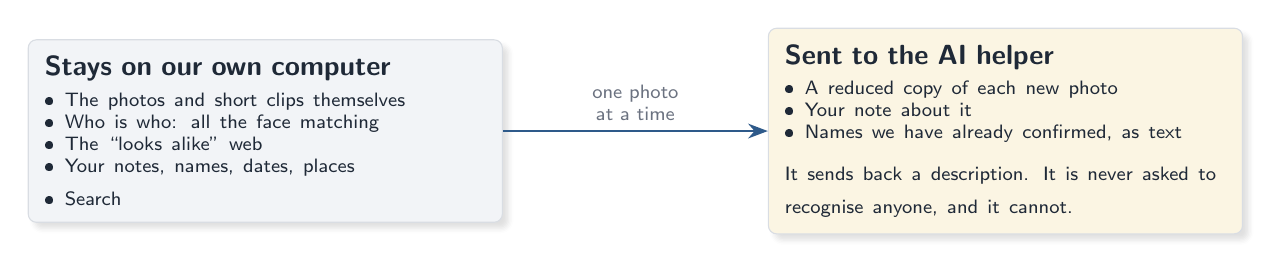
\begin{tikzpicture}
    \node[box,text width=5.6cm,fill=mist,minimum height=2.3cm,align=left] (home) at (0,0) {\textbf{Stays on our own computer}\\[3pt]\scriptsize
      \textbullet\ The photos and short clips themselves\\
      \textbullet\ Who is who: all the face matching\\
      \textbullet\ The ``looks alike'' web\\
      \textbullet\ Your notes, names, dates, places\\
      \textbullet\ Search};
    \node[box,text width=5.6cm,fill=sand!40,minimum height=2.3cm,align=left] (ai) at (9.4,0) {\textbf{Sent to the AI helper}\\[3pt]\scriptsize
      \textbullet\ A reduced copy of each new photo\\
      \textbullet\ Your note about it\\
      \textbullet\ Names we have already confirmed, as text\\[3pt]
      It sends back a description. It is never asked to recognise anyone, and it cannot.};
    \draw[arrow] (home.east) -- node[above,font=\scriptsize,text=muted,align=center,text width=2.4cm]{one photo\\at a time} (ai.west);
  \end{tikzpicture}
  \caption{What leaves the family computer, and what never does.}
\end{figure}

\begin{privacy}
\begin{itemize}
  \item Recognising faces happens entirely on our own computer. Nothing about faces is sent anywhere.
  \item The AI helper only receives photos to write descriptions. It can be switched off for the whole album, and any single upload can be marked ``do not describe''.
  \item Anyone can ask to be left out of face matching. Their existing matches are deleted and no new ones are made.
  \item Children are not matched at all until they are adults, unless a parent turns it on for them.
  \item Every photo and description can be edited or deleted by a family member at any time.
\end{itemize}
\end{privacy}

% ================= Decisions =================
\section{Things for us to decide together}

\begin{enumerate}[leftmargin=2em,itemsep=4pt]
  \item \textbf{Videos.} Clips under about a minute go into the album; anything longer goes on YouTube as unlisted and is linked in. Is a minute the right cut-off, and is everyone comfortable with long videos living on YouTube?
  \item \textbf{The AI helper.} Are we comfortable sending reduced copies of new photos to Anthropic so they can be described and searched? It costs roughly a few cents per photo, and a few hundred dollars once to describe a library of ten thousand old pictures. A cheaper helper writes shorter descriptions for about a fifth of that.
  \item \textbf{Faces.} Is everyone happy with face matching on our own computer, with the opt-out described above, and with children left out until they are adults?
  \item \textbf{How much we have.} A few thousand photos work on the small computer we have. If the shoeboxes add up to a hundred thousand, we need a bigger one.
  \item \textbf{Who does the scanning.} The review screen is designed so one note can cover a whole envelope of prints. Volunteers welcome.
  \item \textbf{Google Photos.} Should we bring our Google Photos libraries over with Takeout, and would each of you connect your Google account for the pick-a-few button?
\end{enumerate}

% ================= Timeline =================

\section{When}

The work is planned in five steps. Each one is useful on its own, so the album keeps working throughout, and we can stop or reorder after any step.

\begin{figure}[H]
  \centering
  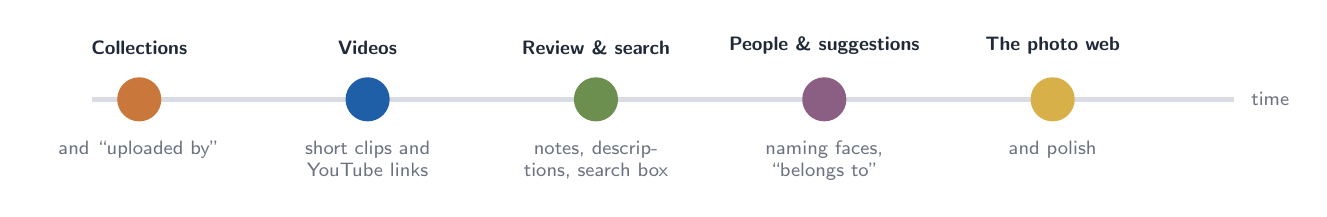
\begin{tikzpicture}
    \draw[line width=2pt,color=line] (0,0) -- (14.5,0);
    \foreach \x/\c/\t/\d in {
      0.6/ph1/Collections/{and ``uploaded by''},
      3.5/ph2/Videos/{short clips and YouTube links},
      6.4/ph3/Review \& search/{notes, descriptions, search box},
      9.3/ph4/People \& suggestions/{naming faces, ``belongs to''},
      12.2/ph5/The photo web/{and polish}} {
      \fill[\c] (\x,0) circle (0.28);
      \node[lbl,anchor=south,align=center,font=\scriptsize\bfseries] at (\x,0.45) {\t};
      \node[mlbl,anchor=north,align=center,text width=2.6cm] at (\x,-0.4) {\d};
    }
    \node[mlbl,anchor=west] at (14.6,0) {\scriptsize time};
  \end{tikzpicture}
  \caption{Five steps, in order. The everyday features arrive with the third and fourth.}
\end{figure}

\vspace{-6pt}
\begin{note}[What we would like from you]
Read this, tell us which of the decisions above you have a view on, and start thinking about which shoebox you would like to scan first. Nothing in the plan is final.
\end{note}

\end{document}
